
\subsection{Gaussian Process}

Gaussian processes (GPs) define a prior over functions that can be updated to a posterior once we have observed data. In a supervised setting, the function gives a mapping between the data points $x_i$ and the target value $y_i$: $y_i = f(x_i)$. Gaussian processes infer a distribution over functions given the data $p(f|x,y)$ and then use it to make predictions given new data. A GP assumes that the function is defined at a finite and arbitrary chosen set of points $x_1,...,x_n$, such that $p(f(x_1),...,f(x_n))$ is jointly Gaussian with mean $\mu(x)$ and covariance $\Sigma(x)$, where $\Sigma_{ij}=\kappa(x_i,x_j)$ and $\kappa$ is a positive definite kernel function.\\

Supervised learning can be divided into regression (prediction of continuous quantities) and classification (prediction of discrete class labels). Consider a simple regression problem:
\begin{equation}
    f(x) = x^{T}w ~~~~ y = f(x) + \epsilon ~~~~ \epsilon \sim N(0,\sigma_{n}^{2})
\end{equation}
Assuming independent and identically distributed noise, we can write down the likelihood function:
\begin{equation}
    p(y|X,w) = \prod_{i=1}^{n}p(y_i|x_i,w) = \prod_{i=1}^{n}\frac{1}{\sqrt{2\pi}\sigma_n}\exp\{-\frac{(y_i - x_{i}^{T}w)^{2}}{2\sigma_{n}^{2}} \} \sim N(Xw, \sigma_{n}^{2}I)
\end{equation}
In Bayesian framework, we need to specify a prior over the parameters: $w \sim N(0,\Sigma_p)$
Writing only the terms of the likelihood and the prior which depend on the weights, we get:
\begin{eqnarray}
   p(w|X,y) &\propto& \exp\{-\frac{1}{2\sigma_{n}^{2}}||y-Xw||^{2}\}\exp\{-\frac{1}{2}w^{T}\Sigma_{p}^{-1}w\} \\
   &\propto& \exp\{-\frac{1}{2}(w-\bar{w})(\frac{1}{\sigma_{n}^{2}}XX^{T}+\Sigma_{p}^{-1})(w-\bar{w})\}\\
   &\sim& N(\frac{1}{\sigma_{n}^{2}}A^{-1}Xy, A^{-1})
\end{eqnarray}
where $A = \sigma_{n}^{-2}XX^{T} + \Sigma_{p}^{-1}$. Thus, we have a closed form posterior distribution over the parameters $w$. To make predictions using this equation, we need to invert the matrix $A$. 
Assuming the observations are noiseless, we want to predict the function outputs $y_{\ast} = f(x_{\ast})$. Consider the following joint GP distribution:
\begin{equation}
\left( \begin{array}{c}
f\\
f_{\ast} \end{array} \right)
\sim
N \bigg(\left( \begin{array}{c}
\mu\\
\mu_{\ast} \end{array} \right),
\left( \begin{array}{cc}
K & K_{\ast}\\
K_{\ast}^{T} & K_{\ast\ast} \end{array} \right) \bigg)
\end{equation}
where $K=\kappa(X,X)$, $K_{\ast}=\kappa(X,X_{\ast})$ and $K_{\ast\ast}=\kappa(X_{\ast}, X_{\ast})$. Using standard rules for conditioning Gaussians, the posterior has the following form:
\begin{eqnarray}
    p(f_{\ast}|X_{\ast}, X, f) &\sim& N(f_{\ast}|\mu_{\ast},\Sigma_{\ast})\\
    \mu_{\ast} &=& \mu(X_{\ast}) + K_{\ast}^{T}K^{-1}(f-\mu(X))\\
    \Sigma_{\ast} &=& K_{\ast\ast} - K_{\ast}^{T}K^{-1}K_{\ast}
\end{eqnarray}

\begin{figure}[tbhp]
    \centering
    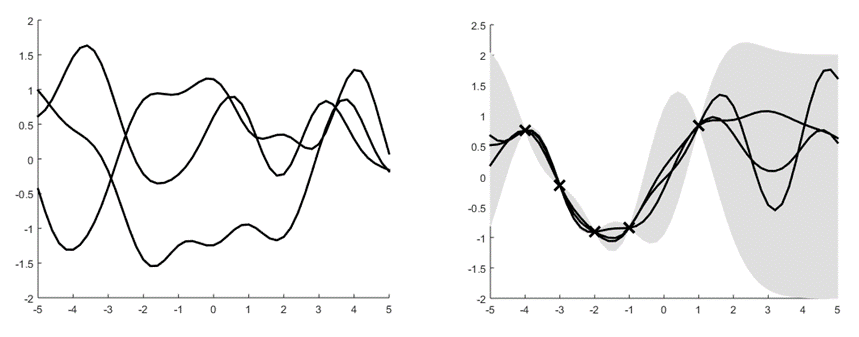
\includegraphics[width=0.8\textwidth, trim={10 10 10 10}]{figures/gp12.png}
    \caption{Gaussian process prior (left) and posterior (right).}
    \label{fig:gp12}
\end{figure}

Figure \ref{fig:gp12} shows three functions drawn at random from a GP prior (left) and GP posterior (right) after observing five data points in the case of noise-free observations. The shaded area corresponds to two times the standard deviation around the mean (95\% confidence region). We can see that the model perfectly interpolates the training data and that the predictive uncertainty increases as we move further away from the observed data.\\

Since our algorithm is defined in terms of inner products in the input space, it can be lifted into feature space by replacing the inner products with $k(x,x^{\prime})$, this is often referred to as the \textit{kernel trick}. The kernel measures similarity between objects and it doesn't require pre-processing them into feature vector format. For a example, a common kernel function is a \textit{radial basis function}:
\begin{equation}
    k(x,x^{\prime}) = \exp\bigg(-\frac{||x-x^{\prime}||^{2}}{2\sigma^2} \bigg)
\end{equation}
In the case of a Gaussian kernel, the feature map lives in an infinite dimensional space. In this case, it is clearly infeasible to explicitly represent the feature vectors. Another commonly used kernel in Gaussian process regression is the \textit{matern kernel}:
\begin{equation}
    \kappa(r) = \frac{2^{1-\nu}}{\Gamma(\nu)}\bigg(\frac{\sqrt{2\nu}r}{l}\bigg)^{\nu}K_{\nu}\bigg(\frac{\sqrt{2\nu}r}{l}\bigg)   
\end{equation}
where $r=||x-x^{\prime}||$, $\nu > 0$, $l > 0$, and $K_{\nu}$ is a modified Bessel function. As $\nu \rightarrow \infty$, this approaches the squared exponential kernel, if $\nu = \frac{1}{2}$, the kernel simplifies to $\kappa(r) = \exp(-r/l)$.\\

Assuming the observations are noisy, $y=f(x)+\epsilon$, where $\epsilon \sim N(0,\sigma_{y}^{2})$, GP is not required to interpolate the data but rather it must be close to the observed data. The covariance of the observed noisy responses is $\mathrm{cov}(y|X) = K + \sigma_{y}^{2}I = K_{y}$, where we assumed that the noise terms were independently added to each observation. Hence, the posterior predictive density is:
\begin{eqnarray}
    p(f_{\ast}|X_{\ast}, X, y) &\sim& N(f_{\ast}|\mu_{\ast},\Sigma_{\ast})\\
    \mu_{\ast} &=& K_{\ast}^{T}K_{y}^{-1}y\\
    \Sigma_{\ast} &=& K_{\ast\ast} - K_{\ast}^{T}K_{y}^{-1}K_{\ast}
\end{eqnarray}
In multiple dimensions, we can write down the \textit{square exponential kernel} as follows:
\begin{equation}
    \kappa_{y}(x_p, x_q) = \sigma_{f}^{2}\exp\big(-\frac{1}{2}(x_p-x_q)^{T}M(x_p-x_q)\big) + \sigma_{y}^{2}\delta_{pq}
\end{equation}
where $M = l^{-2}I$, $l$ is the horizontal scale over which the function changes, $\sigma_{f}^{2}$ controls the vertical scale and $\sigma_{y}^{2}$ is the observation noise variance. 

\begin{figure}[tbhp]
    \centering
    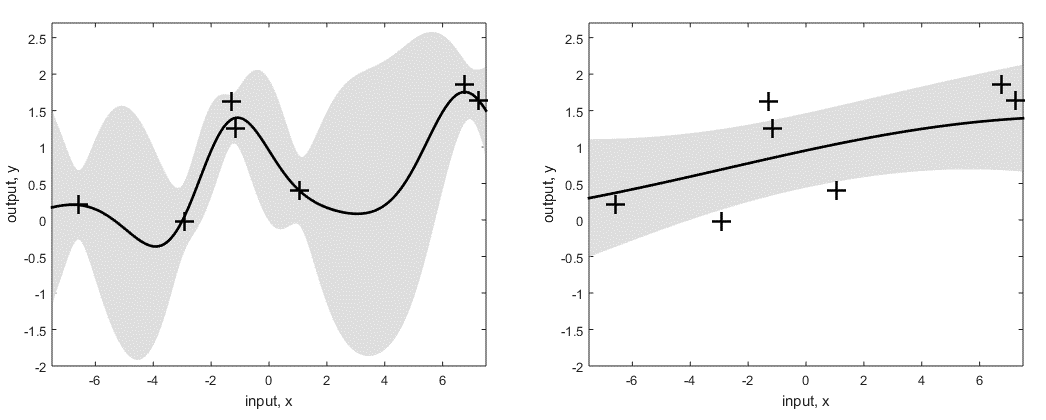
\includegraphics[width=0.8\textwidth, trim={10 10 10 10}]{figures/gp34.png}
    \caption{The effect of varying GP hyperparameters}
    \label{fig:gp34}
\end{figure}
Figure \ref{fig:gp34} shows the importance of choosing kernel hyperparameters and their impact  on GP regression. We fix $\sigma_{f}^{2} = 1$ and plot GP regression after $7$ noisy observations. On the left, the length scale and noise variance were set to $(l,\sigma_{y}^{2}) = (1, 0.2)$. We can see that the mean function appears wiggly and has a small bias due to observation noise. On the right, the kernel parameters were set to $(l,\sigma_{y}^{2}) = (10,0.8)$. The curve is much smoother due to large $l$ and also shows higher observation noise. 

Gaussian Processes (GPs) can be used for classification if the output of a GP is mapped to the range $[0, 1]$. In the binary case, we define the model as $p(y_i|x_i) = \sigma(f(x_i))$, where we let $\sigma(z)=(1+\exp(-z))^{-1}$. As with Bayesian logistic regression, the main difficulty in fitting GP classifier is that the Gaussian prior is not conjugate to the multinoulli likelihood. As a result several approximation algorithms can be used: Gaussian approximation, Expectation Propagation, variational and MCMC. 


\subsection{Dirichlet Process}


The Dirichlet process is a stochastic process used in Bayesian non-parametric models. Each draw from a Dirichlet process is a discrete distribution. For a random distribution $G$ to be distributed according to a DP, its finite dimensional marginal distributions have to be Dirichlet distributed. Let $H$ be a distribution over $\Theta$ and $\alpha$ be a positive real number. We say that $G$ is a Dirichlet process distributed with \textit{base distribution} $H$ and \textit{concentration parameter} $\alpha$ if:

\begin{equation}
    (G(A_1),...,G(A_r)) \sim \mathrm{Dir}(\alpha H(A_1),...,\alpha H(A_r))
\end{equation}
for every finite measurable partition $A_1$,...,$A_r$ of $\Theta$, where Dirichlet distribution is defined as:
\begin{equation}
    p(x_1,...,x_K) = \frac{\Gamma(\sum_k \alpha_k)}{\prod_k \Gamma(\alpha_k)}\prod_{k=1}^{K}x_{k}^{\alpha_k-1}
\end{equation}
The base distribution is the mean of the DP: $E[G(A)] = H(A)$, whereas the concentration parameter is the inverse variance: $V[G(A)] = H(A)(1-H(A))/(\alpha+1)$ for any measureable set $A\subset \Theta$. The larger the $\alpha$, the smaller the variance, and the DP will concentrate more of its mass around the mean.
\begin{figure}[tbhp]
    \centering
    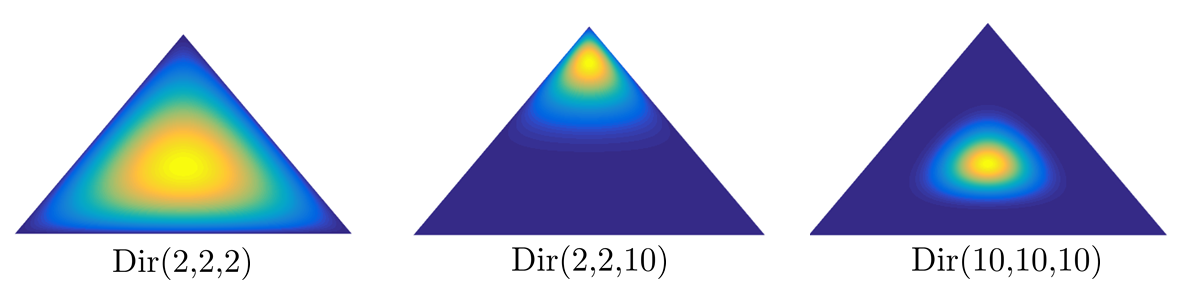
\includegraphics[width=0.8\textwidth, trim={10 10 10 10}]{figures/dir_merged.png}
    \caption{Dirichlet distribution: $\mathrm{Dir}(\alpha_1,\alpha_2,\alpha_3)$ over the simplex.}
    \label{fig:dir_merged}
\end{figure}
Let $\theta_1,...,\theta_n$ be a sequence of independent draws from $G\sim DP(\alpha,H)$. We are interested in the posterior distribution of G given observed values of $\theta_1,...,\theta_n$. Let $n_k$ be the number of observed values in $A_k$, the by conjugacy the Dirichlet and multinomial distributions we have:
\begin{equation}
    (G(A_1),...,G(A_r))|\theta_1,...,\theta_n \sim \mathrm{Dir}(\alpha H(A_1)+n_1,...,\alpha H(A_r)+n_r)
\end{equation}
The posterior is also a DP with an updated concentration parameter and base distribution \cite{Teh2010a}:
\begin{equation}\label{equ:dp_posterior}
    G|\theta_1,...,\theta_n \sim DP(\alpha+n, \frac{\alpha}{\alpha+n}H + \frac{n}{\alpha+n}\frac{\sum_{i=1}^{n}\delta_{\theta_i}}{n})
\end{equation}
Note that the posterior base distribution is a weighted average between the prior base distribution $H$ and the empirical distribution $\frac{1}{n}\sum_{i=1}^{N}\delta_{\theta_i}$. Therefore, $\alpha$ can be interpreted as the strength of the prior. 

\subsection{Construction of the DP}

The Dirichlet Process can be represented in different ways and the representation influences the inference procedure.

\subsubsection{Blackwell-MacQueen Urn Scheme}

The Blackwell-MacQueen Urn Scheme, also commonly known as the Polya urn scheme, provides a way of constructing a sequence of draws $\theta_1, \theta_2,...,\theta_n~\sim G$ where $G\sim DP(\alpha, H)$ without explicitly having to represent $G$. The posterior distribution with $G$ marginalized out and $\theta_1 \sim H$ can be written as:
\begin{equation}\label{equ:urn}
    \theta_{n+1}|\theta_1,...,\theta_n \sim \frac{1}{\alpha+n}\bigg(\alpha H + \sum_{i=1}^{n}\delta_{\theta_i}\bigg)
\end{equation}
The above equation describes a sequential process for drawing $\theta_i$ from $G$, which can be described by the following urn metaphor. First draw $\theta_1 \sim H$, paint a ball with that color and put it in the urn. Then, at each subsequent step $n$, either draw $\theta_n \sim H$ with probability $\alpha/(\alpha + n)$ and put a ball of that color in the urn, or with probability $n/(\alpha + n)$, randomly draw a ball from the urn, set $\theta_n$ to its color, then paint a new ball in that color and return both balls to the urn.

\begin{figure}[tbhp]
    \centering
    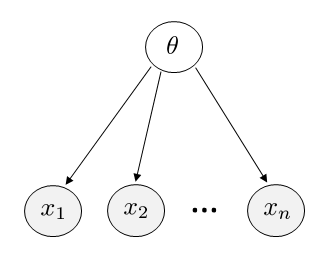
\includegraphics[width=0.3\textwidth, trim={10 10 10 10}]{figures/naive_bayes_gm.png}
    \caption{Naive Bayes graphical model}
    \label{fig:naive_bayes_gm}
\end{figure}

The Blackwell-MacQueen urn model has been used to show the existence of the DP. Starting from (\ref{equ:urn}) we can construct a distribution over draws as follows:
\begin{equation}
    P(\theta_1,...,\theta_n) = \prod_{i=1}^{n}P(\theta_i|\theta_1,...,\theta_{i-1})
\end{equation}
This random sequence is infinitely exchangeable: the probability of generating $\theta_1,...\theta_n$ in that order is equal to the probability of generating them in any alternative order. Thus, for a given permutation $\sigma$, we have
\begin{equation}
    P(\theta_1,...,\theta_n) = P(\theta_{\sigma(1)},...,\theta_{\sigma(2)})
\end{equation}
The strength of infinite exchangeability lies in the following theorem:
\begin{theorem}
(De Finetti, 1930s) A sequence of random variables $x_1, x_2,..,x_n$ is infinitely exchangeable iff for all $n$:
\begin{equation}
    p(x_1,x_2,...,x_n) = \int p(\theta)\prod_{i=1}^{n}p(x_i|\theta)d\theta
\end{equation}
\end{theorem}
Therefore, if we have exchangeable data, there must exist a parameter $\theta$, a likelihood $p(x|\theta)$ and a distribution $P$ on $\theta$ such that conditioned on $\theta$ the observations are independent as shown in Figure \ref{fig:naive_bayes_gm}. In our setting, the prior over the random distribution $p(\theta)$ is the Dirichlet Process $DP(\alpha, H)$, thus establishing existence.

\subsubsection{Chinese Restaurant Process}

Chinese Restaurant Process (CRP) is a discrete-time stochastic process that is based on the clustering property of a DP. Let $\theta_{1}^{\ast},...,\theta_{m}^{\ast}$ be unique values of draws $\theta_1,...,\theta_n$ and $n_k$ be the number of repetitions of $\theta_{k}^{\ast}$. Then, the predictive distribution can be written as:
\begin{equation}
    \theta_{n+1}|\theta_1,...,\theta_n \sim \frac{1}{\alpha+n}\bigg(\alpha H + \sum_{k=1}^{m}n_k \delta_{\theta_{k}^{\ast}}\bigg)
\end{equation}
Notice that $\theta_{k}^{\ast}$ will be repeated in proportion to $n_k$, the number of times it has already been observed. This is a \textit{rich-gets-richer} phenomenon: the larger the cluster, the faster it will grow.
The Chinese Restaurant Process takes its name from a metaphor describing its construction: imagine a Chinese restaurant which has an infinite number of tables, each of which can accomodate an infinite number of clusters. The first customer enters the restaurant and sits at the first table. The $n+1$st customer either joins an already occupied table $k$ with probability proportional to $n_k$ of customers already there or sits at a new table with probability proportional to $\alpha$. Representing customers with integers and tables with clusters, CRP defines a partition on $[n]$. The number of occupied tables $K$ approaches $\alpha \log(n)$ as $n$ approaches infinity. And therefore, DP is a non-parametric prior that favors models whose complexity grows with the amount of data.   

\subsubsection{Stick-Breaking Construction}

The stick breaking construction \cite{sethuraman94} represents draws $G\sim DP(\alpha, H)$ as a weighted sum of atoms (point masses). It is given as follows:
\begin{eqnarray}
    \beta_k \sim \mathrm{Beta}(1,\alpha) ~~~ ~~~~ ~~~~ ~~~~ \theta_{k}^{\ast}\sim H\\
    \pi_k = \beta_k\prod_{l=1}^{k-1}(1-\beta_l) ~~~~ ~~~~ G = \sum_{k=1}^{\infty}\pi_k \delta_{\theta_{k}^{\ast}}
\end{eqnarray}

\begin{figure}[tbhp]
    \centering
    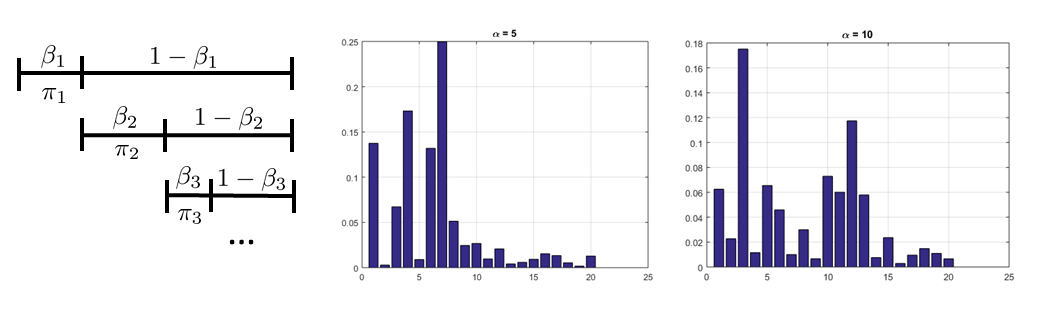
\includegraphics[width=0.8\textwidth, trim={10 10 10 10}]{figures/stick_breaks.png}
    \caption{Stick-Breaking Weights}
    \label{fig:sticks}
\end{figure}

This construction guarantees that $G\sim DP(\alpha, H)$. The name stick-breaking comes from the fact that one can interpret the $\pi_k$ as the lengths broken off a unit length stick as shown in Figure \ref{fig:sticks} for $\alpha=5$ and $\alpha=10$.

\subsection{Hierarchical Dirichlet Process (HDP)}


Hierarchical Dirichlet Processes model problems involving groups of data, where each observation within a group is a draw from a mixture model and mixture components are shared between groups. In each group, the number of components is learned from data using a Dirichlet Process prior. In addition, the base measure for the child Dirichlet processes is itself distributed according to a Dirichlet process. Since a draw from the global DP is a discrete distribution, the group-level DPs share mixture components. 
The HDP model can be summarized as follows and is shown in Figure \ref{fig:hdp_gm}:
\begin{eqnarray}
   G_0 | \gamma, H \sim DP(\gamma, H)\\
   G_j | \alpha, G_0 \sim DP(\alpha, G_0)
\end{eqnarray}
\begin{figure}[tbhp]
    \centering
    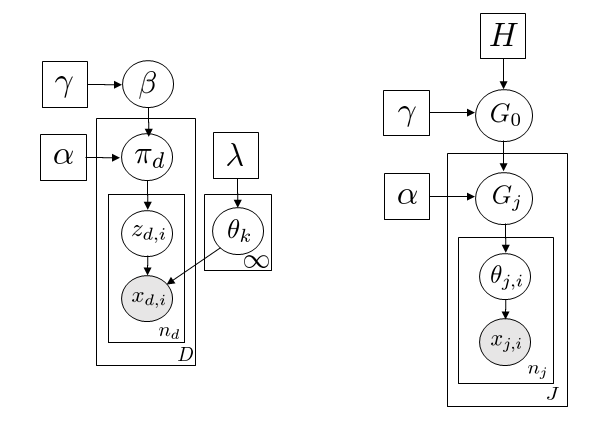
\includegraphics[width=0.6\textwidth, trim={10 10 10 10}]{figures/hdp_gm.png}
    \caption{HDP Graphical Model}
    \label{fig:hdp_gm}
\end{figure}
The distribution $G_0$ varies around the prior $H$, with the amount of variability given by $\gamma$. The actual distribution $G_j$ over $\theta_{j,i}$ in $j^{th}$ group deviates from $G_0$ with the amount of variability given by $\alpha$. If we expect the amount of variability between groups to be different, we can use a separate concentration parameter $\alpha_j$ for each group $j$.\\

Given the global DP prior $G_0$, we can express it using a stick-breaking representation:
$G_0 = \sum_{k=1}^{\infty}\beta_k \delta_{\phi_k}$, where $\phi_k \sim H$ and $\beta_k \sim \mathrm{GEM}(\gamma)$. Since $G_0$ has support at the points $\phi_k$, each $G_j$ has support at these points as well and can be written as: $G_j = \sum_{k=1}^{\infty}\pi_{jk}\delta_{\phi_k}$. The group weights $\pi_j$ are related to global weights $\beta$ as follows \cite{teh2005jasa}:

\begin{eqnarray}
    \beta_{k}^{\prime} \sim \mathrm{Beta}(1,\gamma) ~~~~~~~~ \beta_k = \beta_{k}^{\prime}\prod_{l=1}^{k-1}(1-\beta_{l}^{\prime})\\
    \pi_{jk}^{\prime} \sim \mathrm{Beta}(\alpha\beta_k, \alpha(1-\sum_{l=1}^{k}\beta_l)) ~~~~~~~~ \pi_{jk} = \pi_{jk}^{\prime}\prod_{l=1}^{k-1}(1-\pi_{jl}^{\prime})
\end{eqnarray}

An analog of the Chinese restaurant process for HDPs is the Chinese restaurant franchise (CRF): the metaphor is extended to allow multiple restaurants which share a set of dishes. In this interpretation, each group defines a separate restaurant in which customers (observations) $x_{ji}$ sit at tables (clusters) $t_{ji}$. Each table shares a single dish (parameter) $\theta_{ji}$, which is ordered from a menu $G_0$ shared among restaurants (groups) as shown in Figure \ref{fig:crf}\\
\begin{figure}[thpb]
    \centering
    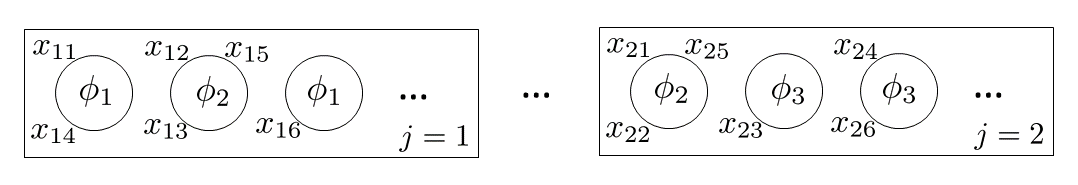
\includegraphics[width=0.8\textwidth, trim={10 10 10 10}]{figures/crf.png}
    \caption{Chinese Restaurant Franchise (CRF). Each restaurant is represented by a rectangle. Customers $x_{ji}$ are seated at tables. At each table a dish $\phi_k$ is served from a global menu.}
    \label{fig:crf}
\end{figure}

Let $\phi_1,...,\phi_K$ denote the $K$ atoms distributed according to $H$: this is the global menu of dishes. Let $\psi_{jt}$ represent table-specific choice of dishes; in particular $\psi_{jt}$ is the dish served at table $t$ in restaurant $j$. Note that each $\theta_{ji}$ is associated with one $\psi_{jt}$ and each $\psi_{jt}$ is associated with one $\phi_k$. In the CRF metaphor, customer $i$ in restaurant $j$ sat at table $t_{ji}$, while table $t$ in restaurant $j$ served dish $k_{jt}$.

The number of tables in restaurant $j$ serving dish $k$ is denoted $m_{jk}$, and the number of customers in restaurant $j$ at table $t$ eating dish $k$ is $n_{jtk}$. Marginal counts are represented with dots. For example, $n_{j..}$ and $m_{j.}$ represent the number of customers and tables, respectively, in restaurant $j$.\\

We can compute the marginals under HDP when $G_0$ and $G_j$ are integrated out using (\ref{equ:dp_posterior}):
\begin{equation}\label{equ:hdp_theta}
    \theta_{ji}|\theta_{j1},...,\theta_{jn},\alpha,G_0 \sim \sum_{t=1}^{m_{j.}} \frac{n_{jt.}}{n+\alpha}\delta_{\psi_{jt}} + \frac{\alpha}{n+\alpha}G_0
\end{equation}
If a term in the first summation is chosen, we set $\theta_{ji}=\psi_{jt}$. If the second term is chosen then we increment $m_{j.}$ by one and draw $\psi_{jm_{j.}}\sim G_0$. To integrate out $G_0$, we can use (\ref{equ:dp_posterior}) again:
\begin{equation}\label{equ:hdp_psi}
    \psi_{jt}|\psi_{11},\psi_{12},...,\psi_{21},...,\gamma,H \sim \sum_{k=1}^{K}\frac{m_{.k}}{m_{..}+\gamma}\delta_{\phi_k} + \frac{\gamma}{m_{..}+\gamma}H
\end{equation}
To summarize, for each $j$ and $i$, we first sample $\theta_{ji}$  using (\ref{equ:hdp_theta}). If a new sample from $G_0$ is needed, we use (\ref{equ:hdp_psi}) to obtain a new sample $\psi_{jt}$.

An on-line variational inference algorithm for Hierarchical Dirichlet Process \cite{wang11a} was used to fit a topic model on the 20newsgroups dataset. The dataset consists of $11,314$ documents and over $100K$ unique tokens. Standard text pre-processing was used including tokenization, stop-word removal and stemming. A compressed dictionary of $4K$ words was constructed by filtering out tokens that appear in less than $5$ documents and more than $50\%$ of the corpus. The top-level truncation was set to $T=20$ topics and the second level truncation was set to $K=8$ topics. The concentration parameters were chosen as $\gamma = 1.0$ at the top-level and $\alpha=0.1$ at the group level to yield a broad range of shared topics that are concentrated at the group level. Figure \ref{fig:hdp_topics} shows a sample of the global level topics inferred by online variational HDP algorithm. We can find topics about autos, politics and for sale items that correspond to the target labels of the 20newsgroups dataset.
\begin{figure}[thpb]
    \centering
    
\includegraphics[width=0.8\textwidth, trim={10 10 10 10}]{figures/hdp_topics.png}
    \caption{Sample of HDP topics inferred using online variational bayes algorithm on 20newsgroups dataset.}
    \label{fig:hdp_topics}
\end{figure}

\subsubsection{HDP Hidden Markov Models}

The Hierarchical Dirichlet Process (HDP) can be used to define a prior distribution on transition matrices over countably infinite state spaces. The HDP-HMM is known is an infinite Hidden Markov Model where the number of states is inferred automatically. To consider a non-parametric variant of the HMM, we must consider a set of DPs, one for each value of the current state. In addition, the DPs must be linked because we want the same set of next states to be reachable from each of the current states. The relates directly to HDP, where the atoms associated with state-conditional DPs are shared.

\begin{figure}[thpb]
    \centering
    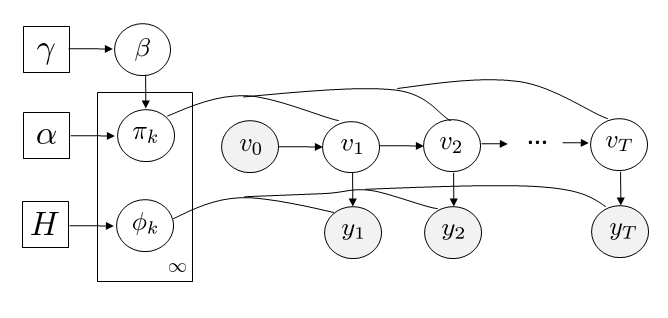
\includegraphics[width=0.6\textwidth, trim={10 10 10 10}]{figures/hdp_hmm_gm.png}
    \caption{HDP-HMM graphical model}
    \label{fig:hdp_hmm_gm}
\end{figure}

We can describe the HDP-HMM model in Figure \ref{fig:hdp_hmm_gm} using the stick-breaking construction. The parameters have the following distribution:
\begin{equation}
    \beta|\gamma \sim \mathrm{GEM}(\gamma) ~~ \pi_k|\alpha,\beta \sim DP(\alpha,\beta) ~~ \phi_k|H \sim H
\end{equation}
for each $k=1,2,...$ while for time steps $t=1,...,T$ the state and observation distributions are:
\begin{equation}
    v_t|v_{t-1}, \pi_k \sim \pi_{v_{t-1}} ~~~~ y_t|v_{t},\phi_k \sim F(\phi_{v_t})
\end{equation}
given a starting state $v_0$. Each $\pi_j$ is a DP draw and is interpreted as the transition distribution from state $j$. The $\pi_j$s are linked through DP draws parameterized by the same discrete measure $\beta$. Therefore, the states are shared between different DP draws. 

Besides Gibbs sampling, one way to compute the posterior for infinite HMM is using a \textit{beam sampling} algorithm \cite{VanSaaTeh2008a}. Beam sampling combines two ideas: slice sampling and dynamic programming to sample whole state trajectories. Slice sampling is applied to limit the number of states to a finite number in each time step of the iHMM. The underlying idea is to limit the beam search to a small number of states so that a good trajectory can be found. Beam sampling is an MCMC method that guarantees convergence to the true posterior.\\

\begin{figure}[thpb]
    \centering
    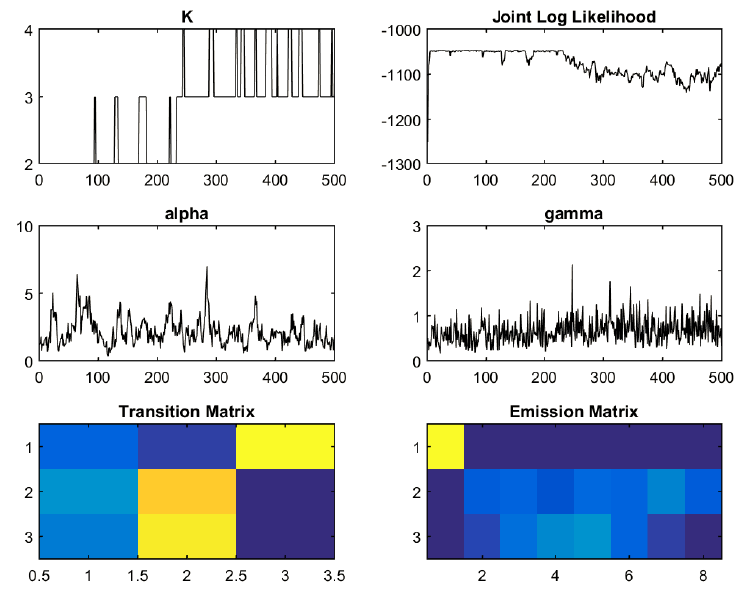
\includegraphics[width=0.7\textwidth, trim={10 10 10 10}]{figures/ihmm_beam.png}
    \caption{HDP-HMM inference results using the beam sampling algorithm \cite{VanSaaTeh2008a}.}
    \label{fig:ihmm_beam}
\end{figure}

Figure \ref{fig:ihmm_beam} shows posterior inference results for synthetically generated time-series data. The ground truth data was generated using $4$ unique states for given transition and emition matrices. From the top-left plot in Figure \ref{fig:ihmm_beam}, we can see that the beam sampler discovered three transition states at iteration $250$. We can also see the samples of $\alpha$ and $\gamma$ concentration parameters for the HDP-HMM as well as the transition and emission matrices. 


\subsection{Dependent Dirichlet Process (DDP)}


The earlier part of Bayesian non-parametric literature focused on problems where a single distribution is assigned a non-parametric prior. However, in many applications, the objective is modelling a collection of distributions used in temporal and spatial processes. The Dirichlet process assumes that observations are exchangeable and therefore the data points have no inherent ordering that influences their labelling. This assumption is invalid for modelling termporal and spatial processes in which the order of data points plays a critical role in creating meaningful clusters.\\

The dependent Dirichlet process (DDP) originally formulated by MacEachern \cite{maceachern99a} provides a non-parametric prior over evolving mixture models. A construction of the DDP built on Poisson process \cite{dhlin10nips} led to the development of the DDP mixture model (DDPMM) which generalizes DPMM by including birth, death and transition processes for the clusters in the model. In addition, a low-variance approximations to DDPMM have been derived leading to a dynamic clustering algorithm \cite{Campbell13_NIPS}.\\

\begin{figure}[thpb]
    \centering
    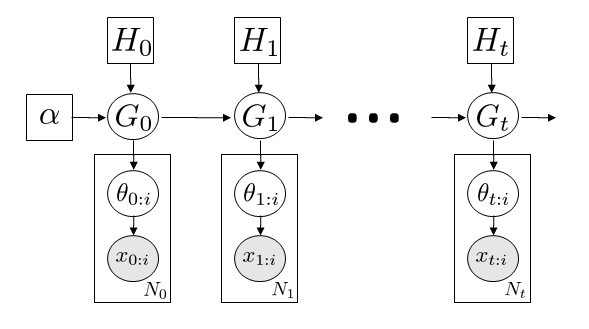
\includegraphics[width=0.6\textwidth, trim={10 10 10 10}]{figures/ddp_gm.png}
    \caption{Dependent Dirichlet Process (DDP) graphical model.}
    \label{fig:ddp_gm}
\end{figure}

Under time-varying setting, it is natural to introduce different DP priors for different time steps as shown in Figure \ref{fig:ddp_gm}. The generative model can be written as:
\begin{eqnarray}
    D_t \sim DP(\alpha, H_t)\\
    \theta_{t:i}|D_t \sim D_t ~~~for i=1,...,n_t,~t=0,...,T\\
    x_{t:i}|\theta_{t:i} \sim F(\theta_{t:i}) ~~~for i=1,...,n_t,~t=0,...,T
\end{eqnarray}

A Poisson-based construction of DDP \cite{dhlin10nips} exploits the connection between Poisson and Dirichlet processes. In particular, by applying operations that preserve \textit{complete randomness} to the underlying Poisson processes: superposition, subsampling and point transition, a new Poisson and therefore a new Dirichlet process is produced. Therefore, a Markov chain of Dirichlet processes can be written as:
\begin{equation}
    D_t = T(S_q(D_{t-1}))\bigoplus H_t, ~~~where H_t \sim DP(\alpha, H)
\end{equation}
where $S_q$ is an acceptance function, $T$ is a probabilistic transition, combined with new terms from innovation process $H_t$ to form $D_t$. 


\subsection{Indian Buffet Process}

The Indian Buffet Process(IBP) is a stochastic process defining a probability distribution over sparse binary matrices with a finite number of rows and an infinite number of columns. This distribution is suitable to use as a prior for models with potentially infinite number of features. The form of the prior ensures that only a finite number of features will be present in any finite set of observations but more features may appear as more data points are observed.\\

Let $Z$ be a $N\times K$ binary matrix indicating the presence or absence of a latent feature. The IBP places the following prior on $Z$ \cite{ibp2011}:
\begin{equation}
    p(Z) = \frac{\alpha^K}{\prod_{i=1}^{N}K_{1}^{(i)}!}\exp\{-\alpha H_N\}\prod_{k=1}^{K}\frac{(N-m_k)!(m_k-1)!}{N!}
\end{equation}
where $K$ is the number of nonzero columns in $Z$, $m_k$ is the number of ones in column $k$ of $Z$, $H_N$ is the $N^{th}$ harmonic number, and $K_h$ is the number of occurences of the non-zero binary vector $h$ among the columns in $Z$. The parameter $\alpha$ controls the expected number of features present in each observation.\\

In the Indian Buffet Process (IBP), the rows of $Z$ correspond to customers and the columns correspond to dishes in an infinitely long buffet. The first customer takes the first $\mathrm{Poisson}(\alpha)$ dishes. The $i$th customer than takes dishes that have been previously sampled with probability $m_k/i$, where $m_k$ is the number of people who have already sampled dish $k$. He also takes $\mathrm{Poisson}(\alpha/i)$ new dishes. Then, $z_{nk}$ is one if customer $n$ tried $k$th dish and zero otherwise.

\begin{figure}[thpb]
    \centering
    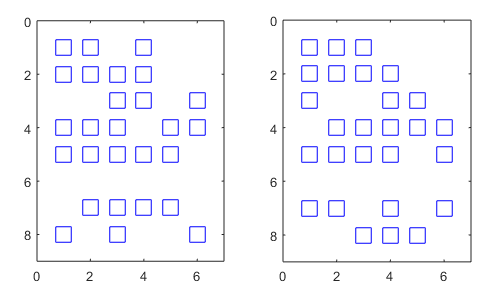
\includegraphics[width=0.5\textwidth, trim={10 10 10 10}]{figures/lof_feature_matrix.png}
    \caption{Original binary feature matrix (left) and its left-ordered form (right)}
    \label{fig:lof}
\end{figure}

This process is infinitely exchangeable for an equivalence class of binary matrices defined by a left-ordered many-to-one function. $lof(Z)$ is obtained by ordering the columns of the binary matrix $Z$ from left to right by the magnitude of the binary number expressed by that column, taking the first row as the most significant bit. The left ordering of a binary matrix is shown in Figure \ref{fig:lof}\\

In this section, we focus on variational inference procedures for the linear-Gaussian likelihood model \cite{DosMilVan2009a}. Let $X$ be a $N\times D$ matrix where each of the $N$ rows contains a $D$-dimensional observation. We focus on a model where $X$ can be approximated as:
\begin{equation}
    X_{N\times D} = Z_{N\times K} \times A_{K\times D} + \epsilon
\end{equation}
where $Z$ is a binary feature matrix, the values for feature $k$ are stored in row $k$ of $A$, and $\epsilon$ is measurement noise.
\begin{figure}[thpb]
    \centering
    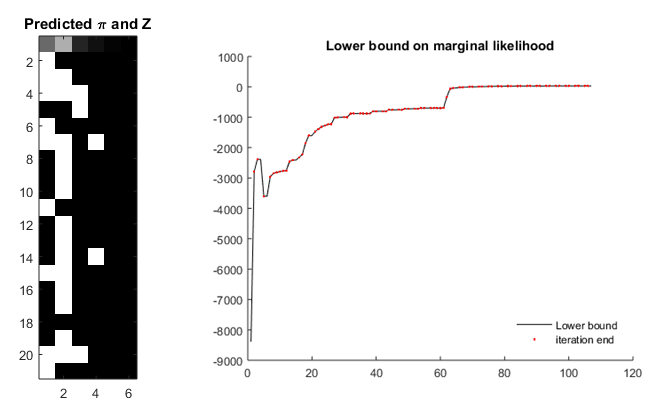
\includegraphics[width=0.6\textwidth, trim={10 10 10 10}]{figures/ibp_z.png}
    \caption{Predicted IBP binary feature matrix $Z$ using variational inference.}
    \label{fig:ibp_z}
\end{figure}
Figure \ref{fig:ibp_z} shows the predicted binary feature matrix $Z$ and lower bound on marginal likelihood using variational inference algorithm for IBP \cite{DosMilVan2009a}. The concentration parameter was set to $\alpha=1$ and the feature truncation level was set to $K=6$. 



\subsection{DPMM}

The Dirichlet Process Mixture Models (DPMM) belong to a class of \textit{infinite mixture models}, in which we do not impose any prior knowledge on the number of clusters $K$. DPMM models learn the number of clusters from the data using a non-parametric prior based on the Dirichlet Process (DP). Automatic model selection leads to computational savings of cross validating the model for multiple values of $K$.\\

Consider the graphical model of the DPMM in Figure \ref{fig:dpmm_gm}.
\begin{figure}[thpb]
    \centering
    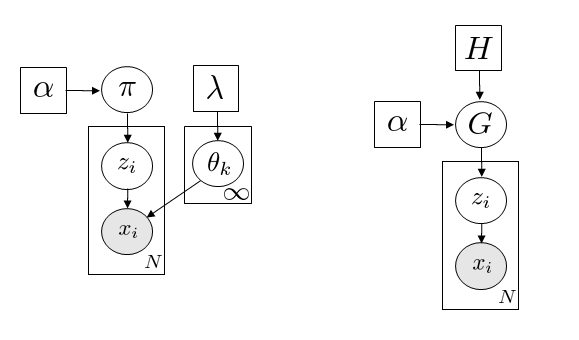
\includegraphics[width=0.6\textwidth, trim={10 10 10 10}]{figures/dpmm_gm.png}
    \caption{DPMM Graphical Model}
    \label{fig:dpmm_gm}
\end{figure}
For each data point $x_i$, there's a corresponding label $z_i$ that assigns the point to one of the clusters with mixture weight $\pi_k$ and parameters $\theta_k = \{\mu_k, \Sigma_k\}$. The generative model can be written as follows:
\begin{eqnarray}
    p(x_i|z_i=k,\theta) &=& p(x_i|\theta_k) \\
    p(z_i=k|\pi) &=& \pi_k \\
    p(\pi|\alpha) &=& \mathrm{Dir}(\pi|\alpha) \\
    p(\theta_k|\beta) &=& \mathrm{NIW}(\mu_k,\Sigma_k|m_0,\kappa_0,\nu_0,S_0)
\end{eqnarray}
An equivalent representation of this model can be written as:
\begin{eqnarray}
    G(\theta) = \sum_{k=1}^{\infty}\pi_k \delta_{\theta_k}
\end{eqnarray}
where $\pi \sim \mathrm{Dir}(\alpha_1,...,\alpha_K)$ and $\theta_k \sim H$. Therefore, $G$ is an infinite mixture of cluster functions of delta functions. In practice, we can construct $G$ using a \textit{stick-breaking construction}:
\begin{eqnarray}
    \beta_k \sim \mathrm{Beta}(1,\alpha)\\
    \pi_k = \beta_k \prod_{l=1}^{k-1}(1-\beta_l) = \beta_k(1-\sum_{l=1}^{k-1}\pi_l)
\end{eqnarray}
This is commonly denoted as $\pi \sim \mathrm{GEM}(\alpha)$. The number of generated mixture components increases with $\alpha$. The hyper-parameter $\alpha$ controls the expected number of clusters:
\begin{eqnarray}
    E[K] = \alpha \times \log(1+n/\alpha)\\
    VAR[K] = \alpha \times \log(1+n/\alpha)
\end{eqnarray}
Thus, the number of clusters grows logarithmically with the number of data points and in direct proportion to $\alpha$ as shown in Figure \ref{fig:dpmm_merged1} 
\begin{figure}[thpb]
    \centering
    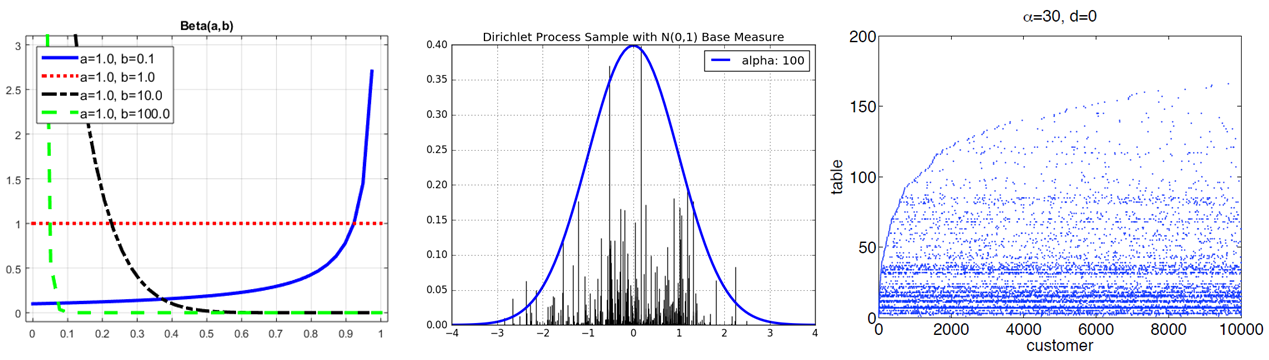
\includegraphics[width=0.9\textwidth, trim={10 10 10 10}]{figures/dp_merged1.png}
    \caption{a) $\mathrm{Beta}(1,\alpha)$ b)DP samples c) DP cluster growth }
    \label{fig:dpmm_merged1}
\end{figure}

\subsection{Fitting a DPMM model}

One way to fit a DPMM is to modify the collapsed Gibbs sampler for a finite mixture model \cite{MurphyML}:
\begin{equation}
    p(z_i=k|z_{-i},x,\alpha,\beta) \propto p(z_i=k|z_{-i},\alpha)p(x_i|x_{-i},z_i=k,z_{-i},\beta)
\end{equation}
The first term is given by the Chinese Restaurant Process (CRP):
\begin{equation}
    p(z_i=k|z_{-i},\alpha) = 
    \begin{cases}
        \frac{N_k}{N+\alpha -1} & \text{if } k \text{ is occupied}\\
        \frac{\alpha}{N+\alpha-1} & \text{if } k \text{ is a new cluster}
    \end{cases}
\end{equation}
The second term is the posterior predictive and can be computed as follows:
\begin{equation}
    p(x_i|x_{-i},z_i=k,z_{-i},\beta) = p(x_i|x_{k\setminus i}, \beta) = \frac{p(x_{k}|\beta)}{p(x_{k\setminus i}|\beta)}
\end{equation}
We can compute both the numerator and the denominator above if we can find an expression for the marginal $p(x)$:
\begin{eqnarray}
    p(x) &=& \int_{\mu} \int_{\Sigma} p(x,\mu,\Sigma) d\mu d\Sigma = \int_{\mu} \int_{\Sigma} p(x|\mu,\Sigma)p(\mu,\Sigma|\beta)d\mu d\Sigma\\
    &=& (2\pi)^{-ND/2}\frac{Z_{NIW}(D,\kappa_N,\nu_N,S_N)}{Z_{NIW}(D,\kappa_0,\nu_0,S_0)} = \pi^{-ND/2}\frac{\kappa_{0}^{D/2}|S_0|^{\nu_0/2}}{\kappa_{N}^{D/2}|S_N|^{\nu_N/2}}\prod_{i=1}^{D}\frac{\Gamma(\frac{\nu_N+1-i}{2})}{\Gamma(\frac{\nu_0+1-i}{2})}
\end{eqnarray}
Therefore, we can write the second term as follows:
\begin{eqnarray}
    \log p(x_i|x_{k\setminus i}) = z(D,N+1,\kappa_{N+1},\nu_{N+1},S_{Ni}) - z(D,N,\kappa_{N},\nu_N,S_N)\\
    z(D,N,\kappa,\nu,S) = -\frac{ND}{2}\log \pi - \frac{D}{2}\log \kappa - \frac{\nu}{2}\log |S| + \sum_{i=1}^{D}\log \Gamma(\frac{\nu+i-1}{2})
\end{eqnarray}
We can summarize, the collapsed Gibbs sampler for an infinite Gaussian mixture model in Algorithm \ref{alg:dpmm_collapsed}.
\begin{algorithm}
\caption{Collapsed Gibbs for DPMM}
\label{alg:dpmm_collapsed}
\begin{algorithmic}[1]
\STATE Initialize labels $z$ 
\STATE for t = 1,2,...,T do 
\STATE ~~~ for i = 1,2,...,N do 
\STATE ~~~ ~~~ remove $x_i$'s statistics from component $z_i$ 
\STATE ~~~ ~~~ delete empty component
\STATE ~~~ ~~~ for k = 1,2,...,K+1 do
\STATE ~~~ ~~~ ~~~ compute $\log p(z_i=k|z_{-i},x,\alpha,\beta) \sim$
\STATE ~~~ ~~~ ~~~ $\log p(z_i = k|z_{-i},\alpha) + \log p(x_i|x_{k\setminus i},\beta)$
\STATE ~~~ ~~~ sample $z_i = k_{new}$ from $p(z_i=k|z_{-i},x,\alpha,\beta)$
\STATE ~~~ ~~~ create a new cluster if $z_i = K+1$
\STATE ~~~ ~~~ add $x_i$'s statistics to component $z_i = k_{new}$ 
\STATE ~~~ end for
\STATE end for
\end{algorithmic}
\end{algorithm}

Figure \ref{fig:dp_results} shows the clustering results of DPMM collapsed gibbs sampler with Gaussian base measure and $\alpha=1$ after $100$ iterations on a synthetic dataset of $1K$ points in 2D. The sampler was initialized with $K_{init}=2$ clusters and correctly identified all $5$ clusters in the data.

\begin{figure}[thpb]
    \centering
    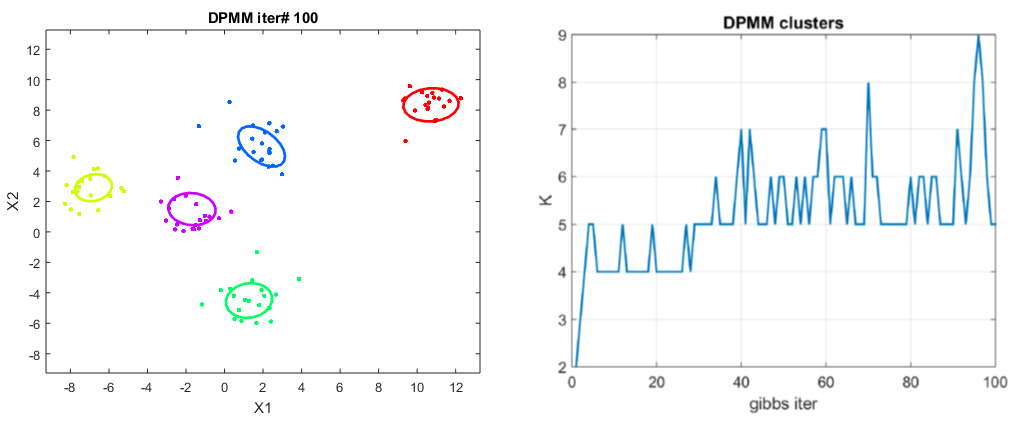
\includegraphics[width=0.8\textwidth, trim={10 10 10 10}]{figures/dp_results.png}
    \caption{DPMM Clustering Results for Gaussian data}
    \label{fig:dp_results}
\end{figure}

Figure \ref{fig:dp_results2} shows the clustering results of DPMM on categorical data. Documents from a reduced NIPS dataset with 300 docs, 5K vocab and 130K words were grouped into $11$ clusters. The top words for the first $4$ clusters are displayed in Figure \ref{fig:dp_results2}. The results indicate meaningful division of articles by topics about neural networks, gaussian mixtures, computer vision and reinforcement learning. The gibbs sampler was initialized with $K_{init}=2$ and $\alpha=1$ and coverged after $20$ iterations through the corpus.   

\begin{figure}[thpb]
    \centering
    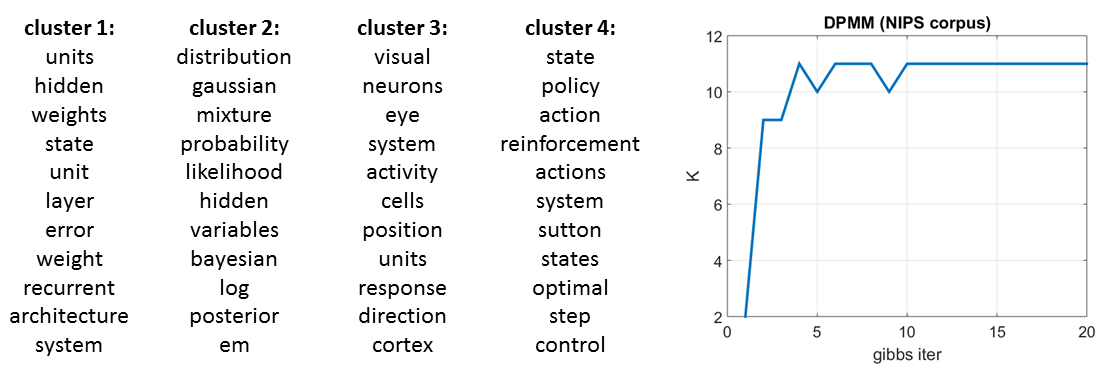
\includegraphics[width=0.8\textwidth, trim={10 10 10 10}]{figures/dp_results2.png}
    \caption{DPMM Clustering Results for Categorical data}
    \label{fig:dp_results2}
\end{figure}



